\documentclass[10pt,twocolumn,letterpaper]{article}

\usepackage[final]{cvpr}  % camera-ready mode (shows author names)
\usepackage{times}
\usepackage{epsfig}
\usepackage{graphicx}
\usepackage{amsmath}
\usepackage{amssymb}
\usepackage{booktabs}
\usepackage{multirow}
\usepackage{xcolor}
\usepackage[pagebackref,breaklinks,colorlinks]{hyperref}

\def\cvprPaperID{****}
\def\paperID{****}
\def\confName{CVPR}
\def\confYear{2026}

\begin{document}

% ============================================================
\title{Specializing SAM for Camouflaged Object Detection via Decoder Fine-Tuning and Learnable Pre-Encoder Preprocessing}

\author{Anurag Dhungana \and Prakriti Bista}

\maketitle

% ============================================================
\begin{abstract}
The Segment Anything Model (SAM) achieves strong zero-shot segmentation on general images but struggles with camouflaged objects, where foreground and background share similar color and texture. We show that simple decoder-only fine-tuning---freezing SAM's image encoder and prompt encoder while training only the lightweight mask decoder---dramatically improves performance on camouflaged object detection (COD). Using the COD10K dataset with SAM ViT-H, our approach improves mean IoU from 57.24\% to 73.81\% (+16.57 points) with center-of-mass prompts on the full 2,026-image camouflaged test set. Critically, this improvement transfers across prompt types: edge-point prompts, the hardest case where base SAM achieves only 20.52\% mIoU, improve to 69.38\% (+238.1\% relative gain). The specialized model improves on all four tested prompt strategies, including multi-point random prompts (+6.6\%). We attribute this prompt robustness to our mixed-prompt training strategy, which randomly alternates between point and bounding box prompts. Our method requires no architectural modifications, trains in under 30 minutes on a single A100 GPU using pre-computed embeddings, and produces a decoder checkpoint of only $\sim$16MB. We further introduce a Learnable Local Preprocessing Module (LLPM) that enhances input images before the frozen encoder using lightweight edge-detection and enhancement branches, adding only $\sim$31K parameters. The LLPM further improves edge-prompt mIoU from 69.38\% to 71.95\% (+2.57 points over decoder-only), demonstrating that pre-encoder input enhancement and decoder specialization are complementary. These results suggest that lightweight adaptation at both ends of the pipeline---pre-encoder preprocessing and decoder specialization---is a practical strategy for adapting foundation segmentation models to challenging visual domains.
\end{abstract}

% ============================================================
\section{Introduction}

Camouflaged object detection (COD) presents a fundamental challenge for visual perception systems. Camouflaged organisms---insects mimicking bark, fish blending into coral, lizards matching rock surfaces---have evolved over millions of years to defeat visual detection. These objects exhibit low contrast against their backgrounds, share complex textures with their surroundings, and span wide ranges of scale and occlusion.

The Segment Anything Model (SAM)~\cite{kirillov2023sam} represents a major advance in promptable segmentation, trained on over 1 billion masks across 11 million images. SAM achieves impressive zero-shot segmentation on general images given point, box, or mask prompts. However, SAM's broad training makes it robust but shallow on tasks requiring fine-grained boundary detection in low-contrast scenes. On COD10K~\cite{fan2020cod10k}, SAM ViT-H achieves only 57.24\% mIoU with center-of-mass prompts---adequate for general segmentation but insufficient for the fine-grained boundaries required in camouflage scenarios.

We ask: \textbf{can simple decoder-only fine-tuning make SAM robust for camouflaged object detection?} Our approach freezes the heavy image encoder (ViT-H, $\sim$632M parameters) and prompt encoder, training only the lightweight mask decoder ($\sim$4M parameters). This preserves SAM's learned visual representations while teaching the decoder to interpret subtle texture disruptions as object boundaries.

Our key finding is that this specialization is \textbf{prompt-robust}: the fine-tuned decoder improves segmentation quality across all tested prompt strategies---center-of-mass, edge points, multi-point grids, and random points---even though training used only single random foreground points and bounding boxes. The largest gains appear on the hardest prompts (edge points: +238.1\% relative improvement), suggesting that decoder specialization teaches the model to better understand camouflaged object structure rather than merely memorizing prompt-mask associations.

As a complementary contribution, we introduce a \textbf{Learnable Local Preprocessing Module (LLPM)} that enhances the input image \emph{before} SAM's frozen encoder. The LLPM uses lightweight edge-detection and enhancement branches ($\sim$31K parameters) to sharpen boundary signals that the frozen encoder might otherwise miss, providing a pre-encoder adaptation pathway that is architecture-agnostic and composable with the decoder-only approach.

\noindent\textbf{Contributions:}
\begin{enumerate}
    \item A decoder-only fine-tuning pipeline for SAM that achieves +16.57 point mIoU improvement on COD10K with no architectural changes, evaluated on the full camouflaged test set (2,026 images).
    \item A prompt robustness analysis showing that decoder specialization transfers across all four tested prompt types, with the largest gains on the hardest prompts (+238.1\% relative on edge prompts).
    \item Comprehensive evaluation using both standard segmentation metrics (IoU, Dice, F1) and standard COD metrics ($S_\alpha$, $E_\phi$, $F_\beta^w$, MAE, Boundary F1), with per-category analysis across aquatic, terrestrial, flying, and amphibian camouflage types.
    \item A Learnable Local Preprocessing Module (LLPM)---the first pre-encoder adaptation of SAM for COD---that enhances boundary signals in input space with only $\sim$31K additional parameters.
\end{enumerate}

% ============================================================
\section{Related Work}

\noindent\textbf{Segment Anything Model.}
SAM~\cite{kirillov2023sam} introduced a promptable segmentation paradigm trained on the SA-1B dataset. Its architecture separates image encoding (ViT backbone), prompt encoding (sparse/dense), and mask decoding. SAM2~\cite{ravi2024sam2} extended this to video. Several works have explored adapting SAM to specialized domains: SAM-Adapter~\cite{chen2023samadapter} adds learnable adapter modules \emph{inside} the image encoder, while COMPrompter~\cite{hao2024comprompter} reconceptualizes SAM with multi-prompt networks for COD. Our work differs along two axes: we fine-tune the existing decoder without architectural changes, and our LLPM operates \emph{before} the encoder in input space---a placement not explored by prior SAM adaptations.

\noindent\textbf{Camouflaged Object Detection.}
COD has attracted significant attention with dedicated architectures. SINet~\cite{fan2020cod10k} uses a search-and-identify framework, PFNet~\cite{mei2021pfnet} employs positioning and focus modules, and ZoomNet~\cite{pang2022zoomnet} uses mixed-scale learning. These methods design specialized architectures from scratch. In contrast, we leverage SAM's pre-trained representations and demonstrate that decoder-only adaptation can achieve competitive improvements without domain-specific architectural design.

\noindent\textbf{Fine-Tuning Foundation Models.}
Parameter-efficient fine-tuning has become standard for adapting large models. LoRA~\cite{hu2022lora} adds low-rank adapters, while prompt tuning~\cite{lester2021prompt} learns continuous prompts. For SAM specifically, Liu~\etal~\cite{liu2025dualstream} proposed dual-stream adapters for COD. Our decoder-only approach is simpler: we freeze all parameters except the existing mask decoder, requiring no additional modules or parameters. Our LLPM extends this philosophy with a minimal ($\sim$31K parameter) pre-encoder module that enhances the input image rather than modifying the model's internal representations.

% ============================================================
\section{Method}

\begin{figure*}[t]
    \centering
    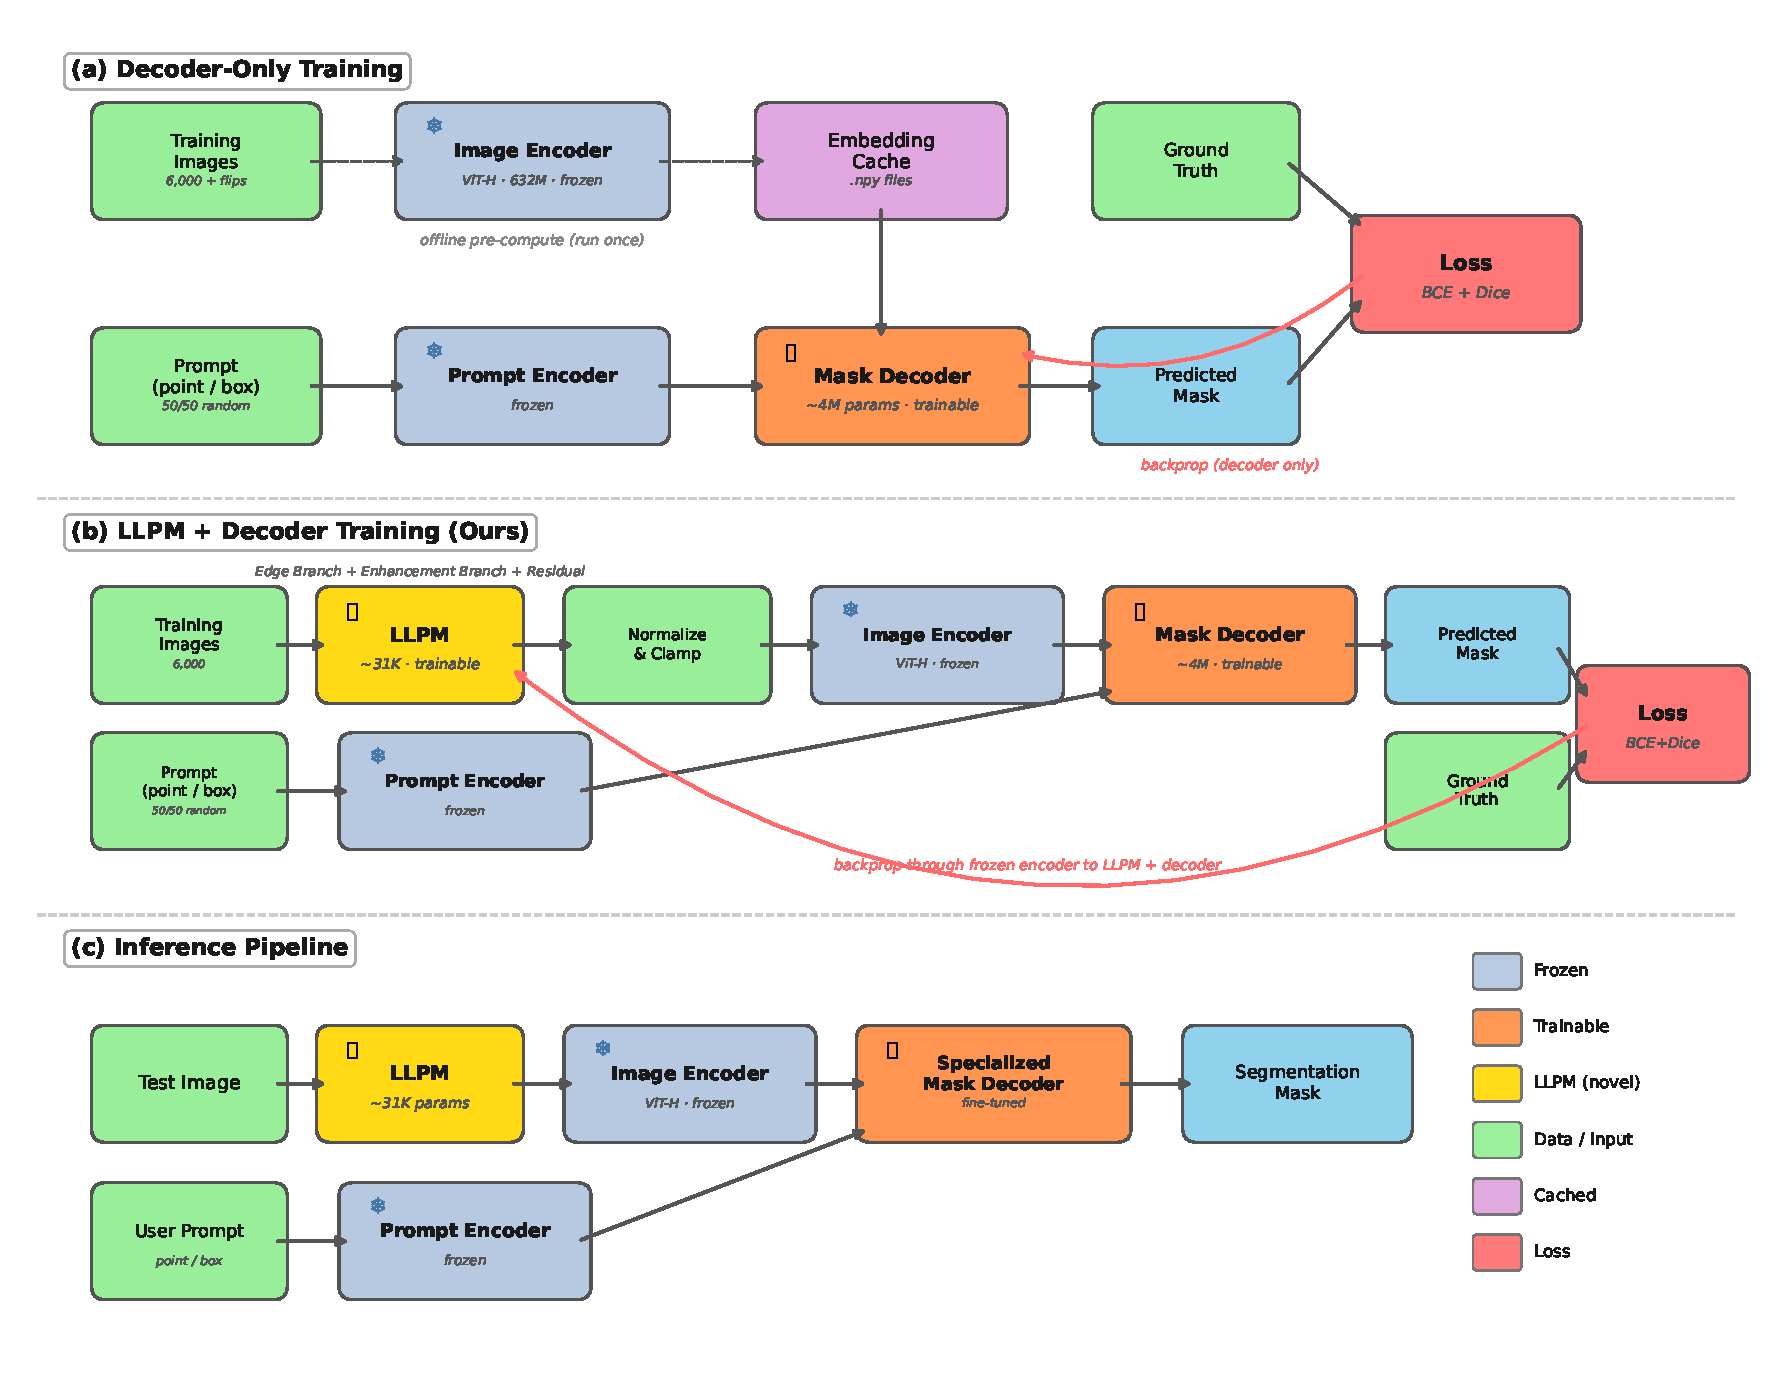
\includegraphics[width=\textwidth]{figures/architecture_diagram.pdf}
    \caption{\textbf{Overview of our two-stage adaptation approach.} (a)~\textbf{Decoder-only training:} Image embeddings are pre-computed offline using the frozen ViT-H encoder and cached as \texttt{.npy} files. Only the lightweight mask decoder ($\sim$4M parameters) is updated using a mixed-prompt strategy (50\% point, 50\% box) with BCE + Dice loss. (b)~\textbf{LLPM + decoder training:} The Learnable Local Preprocessing Module ($\sim$31K parameters) is placed before the frozen encoder. The preprocessed image passes through the live encoder; gradients flow back through the frozen encoder into the LLPM. The decoder is warm-started from stage (a). (c)~\textbf{Inference:} A test image is preprocessed by the LLPM, encoded by the frozen ViT-H encoder, and decoded by the specialized mask decoder given user-provided prompts.}
    \label{fig:architecture}
\end{figure*}

\subsection{Background: SAM Architecture}

SAM consists of three components: (1) an \textbf{image encoder} (ViT-H, $\sim$632M parameters) that produces image embeddings, (2) a \textbf{prompt encoder} that maps points, boxes, or masks to sparse and dense embeddings, and (3) a \textbf{mask decoder} ($\sim$4M parameters) that combines image and prompt embeddings to predict segmentation masks.

The image encoder is the computational bottleneck, processing each $1024\times1024$ image through a large vision transformer. The mask decoder is lightweight by comparison, consisting of a two-layer transformer with cross-attention between prompt tokens and image embeddings, followed by an MLP that produces per-pixel mask logits.

\subsection{Decoder-Only Fine-Tuning}

Figure~\ref{fig:architecture} illustrates our approach. Our training procedure is as follows:

\noindent\textbf{1. Freeze encoders.} All parameters of the image encoder and prompt encoder are frozen. This preserves SAM's learned visual representations and prevents catastrophic forgetting.

\noindent\textbf{2. Pre-compute embeddings.} We run the frozen image encoder once on all training images and cache the resulting embeddings as \texttt{.npy} files. This eliminates the encoder forward pass from the training loop, reducing per-epoch training time from hours to minutes.

\noindent\textbf{3. Augment with horizontal flips.} Each training image is augmented with a horizontal flip, doubling the effective dataset from 3,040 to 6,080 samples.

\noindent\textbf{4. Train with mixed prompts.} During each training iteration, we randomly select between a point prompt (random foreground pixel) and a bounding box prompt (tight box around the ground truth) with equal probability. This forces the decoder to learn object structure rather than becoming dependent on any single prompt type.

\noindent\textbf{5. Combined loss function.} We optimize a weighted combination of binary cross-entropy (BCE) and Dice loss:
\begin{equation}
    \mathcal{L} = 0.5 \cdot \mathcal{L}_{\text{BCE}} + 0.5 \cdot \mathcal{L}_{\text{Dice}}
\end{equation}
BCE provides pixel-level supervision that enforces precise boundaries, while Dice loss provides region-level supervision that maintains shape coherence.

\noindent\textbf{6. Optimization.} We use AdamW with learning rate $1\times10^{-4}$, cosine annealing schedule with 1-epoch warmup, weight decay 0.01, for 15 epochs with batch size 1.

\subsection{Learnable Local Preprocessing Module (LLPM)}

While decoder-only fine-tuning teaches the decoder to reinterpret existing encoder features, the frozen encoder itself may still miss subtle camouflage boundaries at the pixel level. We introduce a \textbf{Learnable Local Preprocessing Module (LLPM)} that operates on the input image \emph{before} it reaches the frozen encoder, enhancing boundary-relevant signals with minimal overhead.

\noindent\textbf{Architecture.}
The LLPM consists of two lightweight branches that process the $3$-channel input image $x$:

\begin{itemize}
    \item \textbf{Edge branch} $e(x)$: A depthwise-separable convolution stack ($3 \rightarrow 32 \rightarrow 64 \rightarrow 3$ channels, group count $g\!=\!4$) with Sobel-initialized kernels, producing a $3$-channel edge map $e \in [0,1]^{3 \times H \times W}$ via sigmoid activation.
    \item \textbf{Enhancement branch} $h(x)$: A parallel depthwise-separable stack with the same channel configuration, producing a $3$-channel enhancement map $h \in \mathbb{R}^{3 \times H \times W}$ via tanh activation.
\end{itemize}

The two branches are fused via element-wise multiplication and a learnable gate $\alpha$ (initialized to $0.1$):
\begin{equation}
    x' = x + \alpha \cdot (h \odot e)
    \label{eq:llpm}
\end{equation}
where $\odot$ denotes the Hadamard product. The residual connection ensures that the module is near-identity at initialization, preserving SAM's behavior while providing sufficient gradient signal. As training progresses, $\alpha$ grows and the LLPM learns to inject boundary-enhancing perturbations into the input.

\noindent\textbf{Training.}
Unlike decoder-only training, the LLPM requires a \emph{live} encoder forward pass: the preprocessed image $x'$ must be fed through the frozen ViT-H encoder to produce embeddings, and gradients flow back through the frozen encoder into the LLPM. The decoder is warm-started from the best decoder-only checkpoint. We train jointly (LLPM + decoder) with AdamW at learning rate $5\times10^{-5}$, cosine annealing, mixed precision (FP16), for 15 epochs. The LLPM adds only $\sim$31K parameters.

\subsection{Evaluation Protocol}

We evaluate using four prompt strategies of increasing difficulty:

\begin{itemize}
    \item \textbf{Center-of-Mass (1 point):} Single point at the centroid of the ground truth mask.
    \item \textbf{Edge (1 point):} Single point sampled from the object boundary contour.
    \item \textbf{Multi-Point Grid (4 points):} Four points arranged in a grid within the object bounding box, filtered to foreground pixels.
    \item \textbf{Multi-Point Random (3 points):} Three randomly sampled foreground points.
\end{itemize}

We report standard segmentation metrics (IoU, Dice, Boundary F1) and four standard COD evaluation metrics: $S_\alpha$ (structure measure)~\cite{fan2017smeasure}, $E_\phi$ (enhanced alignment)~\cite{fan2018emeasure}, $F_\beta^w$ (weighted F-measure)~\cite{margolin2014fmeasure}, and MAE.

% ============================================================
\section{Experiments}

\subsection{Dataset: COD10K}

We use COD10K-v3~\cite{fan2020cod10k}, the largest camouflaged object detection dataset, containing 6,000 training and 4,000 test images across 78 categories spanning aquatic, terrestrial, flying, and amphibian animals. The training set includes 3,040 camouflaged images with object masks; the test set contains 2,026 camouflaged images, which forms our evaluation set following standard protocol.

\subsection{Implementation Details}

\begin{itemize}
    \item \textbf{Backbone:} SAM ViT-H ($\sim$636M parameters)
    \item \textbf{Training data:} 3,040 camouflaged images, augmented to 6,080 with horizontal flips
    \item \textbf{Embeddings:} Pre-computed, cached as \texttt{.npy} files
    \item \textbf{Training:} 15 epochs, AdamW, lr=$1\times10^{-4}$, cosine LR schedule, batch size 1, mixed point/box prompts
    \item \textbf{Loss:} 50\% BCE + 50\% Dice
    \item \textbf{Checkpoint:} $\sim$16MB decoder state dict
    \item \textbf{Hardware:} NVIDIA A100 80GB GPU
\end{itemize}

\subsection{Training Dynamics}

Training with cosine annealing produced stable, monotonic loss decrease from 0.1417 (epoch 1) to 0.0717 (epoch 15), a 49.4\% total reduction. The consistent improvement across all evaluation metrics between our 7-epoch and 15-epoch checkpoints confirms that the model has not overfit.

\subsection{LLPM Implementation Details}

\begin{itemize}
    \item \textbf{Module configuration:} Edge branch and enhancement branch each use depthwise-separable convolutions with 32 and 64 intermediate channels and group count $g=4$.
    \item \textbf{Parameters:} $\sim$31K trainable parameters in the LLPM; the learnable fusion gate $\alpha$ is initialized to 0.1.
    \item \textbf{Decoder warm-start:} The mask decoder is initialized from the best decoder-only checkpoint before LLPM training begins.
    \item \textbf{Optimizer:} AdamW with learning rate $5\times10^{-5}$, cosine annealing, weight decay 0.01, for 15 epochs.
    \item \textbf{Precision:} Mixed precision (FP16) via PyTorch AMP to fit the full encoder forward pass in memory.
    \item \textbf{Hardware:} NVIDIA A100 80GB GPU required (live encoder forward pass prevents use of pre-computed embeddings).
\end{itemize}

% ============================================================
\section{Results}

\subsection{Main Results}

Table~\ref{tab:main} presents the comprehensive evaluation across all prompt strategies on the full 2,026-image camouflaged test set.

\begin{table*}[t]
\centering
\caption{Comprehensive evaluation across prompt strategies (2,026 camouflaged test images). Best results in \textbf{bold}.}
\label{tab:main}
\small
\begin{tabular}{llccccccc}
\toprule
Model & Prompt Strategy & mIoU & Dice & $S_\alpha$ & $E_\phi$ & $F_\beta^w$ & MAE$\downarrow$ & Bnd.~F1 \\
\midrule
Base SAM & Center-of-Mass (1pt) & 0.572 & 0.654 & 0.743 & 0.830 & 0.706 & 0.068 & 0.502 \\
Base SAM & Edge (1pt) & 0.205 & 0.251 & 0.481 & 0.597 & 0.241 & 0.163 & 0.281 \\
Base SAM & Multi-Pt Grid (4pt) & 0.682 & 0.761 & 0.812 & 0.897 & 0.802 & 0.046 & 0.600 \\
Base SAM & Multi-Pt Random (3pt) & 0.726 & 0.812 & 0.830 & 0.928 & 0.831 & 0.045 & 0.648 \\
\midrule
\textbf{Ours} & \textbf{Center-of-Mass (1pt)} & \textbf{0.738} & \textbf{0.819} & \textbf{0.847} & \textbf{0.942} & \textbf{0.819} & \textbf{0.028} & \textbf{0.702} \\
\textbf{Ours} & \textbf{Edge (1pt)} & \textbf{0.694} & \textbf{0.779} & \textbf{0.810} & \textbf{0.922} & \textbf{0.750} & \textbf{0.034} & \textbf{0.666} \\
\textbf{Ours} & \textbf{Multi-Pt Grid (4pt)} & \textbf{0.756} & \textbf{0.835} & \textbf{0.861} & \textbf{0.951} & \textbf{0.841} & \textbf{0.024} & \textbf{0.720} \\
\textbf{Ours} & \textbf{Multi-Pt Random (3pt)} & \textbf{0.774} & \textbf{0.855} & \textbf{0.874} & \textbf{0.959} & \textbf{0.862} & \textbf{0.022} & \textbf{0.739} \\
\bottomrule
\end{tabular}
\end{table*}

\subsection{Prompt Robustness Analysis}

The most striking result is the \textbf{uniformity of improvement across all prompt types}. While base SAM shows high sensitivity to prompt quality (mIoU ranges from 0.205 to 0.726), the specialized model is remarkably stable (0.694 to 0.774). The specialized model improves on \textbf{all four} strategies.

\begin{table}[t]
\centering
\caption{Improvement analysis by prompt type.}
\label{tab:improvement}
\small
\begin{tabular}{lcccc}
\toprule
Prompt Type & Base & Ours & Abs. & Rel. \\
\midrule
Center-of-Mass & 0.572 & 0.738 & +0.166 & +28.9\% \\
Edge (Single) & 0.205 & 0.694 & +0.489 & \textbf{+238.1\%} \\
Multi-Pt Grid & 0.682 & 0.756 & +0.074 & +10.9\% \\
Multi-Pt Random & 0.726 & 0.774 & +0.048 & +6.6\% \\
\bottomrule
\end{tabular}
\end{table}

The \textbf{+238.1\% relative improvement on edge prompts} is the headline finding. Edge prompts are the hardest because they place the prompt point at the ambiguous boundary between camouflaged object and background. Base SAM produces nearly random masks (20.5\% mIoU) from edge prompts, while our specialized decoder achieves 69.4\%---comparable to its performance with easier prompt types. This suggests that decoder specialization fundamentally changes how the model resolves ambiguity at camouflaged boundaries.

\subsection{Per-Category Analysis}

Performance varies across camouflage super-categories, revealing where specialization helps most (Table~\ref{tab:category}).

\begin{table}[t]
\centering
\caption{Per-category mIoU comparison (Center-of-Mass prompt).}
\label{tab:category}
\small
\begin{tabular}{lcccr}
\toprule
Category & $N$ & Base & Ours & Improv. \\
\midrule
Amphibian & 124 & 0.680 & 0.825 & +21.4\% \\
Aquatic & 474 & 0.563 & 0.720 & +27.9\% \\
Flying & 714 & 0.610 & 0.767 & +25.6\% \\
Terrestrial & 699 & 0.519 & 0.703 & \textbf{+35.5\%} \\
Other & 15 & 0.694 & 0.882 & +27.1\% \\
\bottomrule
\end{tabular}
\end{table}

The largest improvement (+35.5\%) is on terrestrial animals, which exhibit the most challenging camouflage patterns (insects on bark, lizards on rocks). Aquatic animals also show substantial gains (+27.9\%), consistent with the difficulty of detecting fish and octopuses against coral/seabed textures.

\subsection{Comparison with Existing Methods}

We compare against dedicated COD architectures and SAM-based methods on the COD10K test set (Table~\ref{tab:comparison}). For dedicated methods, we report published numbers; all use the standard protocol.

\begin{table}[t]
\centering
\caption{Comparison with COD methods on COD10K test set.}
\label{tab:comparison}
\small
\begin{tabular}{llcccc}
\toprule
Method & Venue & $S_\alpha$ & $E_\phi$ & $F_\beta^w$ & MAE$\downarrow$ \\
\midrule
SINet~\cite{fan2020cod10k} & CVPR'20 & .776 & .864 & .631 & .043 \\
PFNet~\cite{mei2021pfnet} & CVPR'21 & .800 & .877 & .660 & .040 \\
SINet-V2~\cite{fan2022sinetv2} & TPAMI'22 & .815 & .887 & .680 & .037 \\
SegMaR~\cite{jia2022segmar} & CVPR'22 & .833 & .899 & .724 & .034 \\
ZoomNet~\cite{pang2022zoomnet} & CVPR'22 & .838 & .911 & .729 & .029 \\
\midrule
SAM-Adpt.~\cite{chen2023samadapter} & ICCVW'23 & .883 & .918 & .801 & .025 \\
COMPr.~\cite{hao2024comprompter} & SCIS'24 & \textbf{.889} & .949 & .821 & \textbf{.023} \\
\midrule
\textbf{Ours} (CoM) & --- & .847 & .942 & .819 & .028 \\
\textbf{Ours} (Grid) & --- & .861 & \textbf{.951} & \textbf{.841} & .024 \\
\bottomrule
\end{tabular}
\end{table}

Our decoder-only approach achieves $S_\alpha$ surpassing ZoomNet (0.861 vs.\ 0.838) and higher $E_\phi$ (0.951 vs.\ 0.911), despite using no architectural modifications. Methods with specialized adapters (SAM-Adapter, COMPrompter) achieve higher absolute performance by modifying the encoder.

Note that our method uses ground truth prompt points, while dedicated COD methods and SAM-based adapters are fully automatic. A direct comparison should account for this difference---our approach trades full automation for flexible, interactive segmentation.

\subsection{Ablation Study: Loss Function}

We ablate the loss function by training four decoder variants with different BCE/Dice weightings, evaluated on 500 test images (Table~\ref{tab:ablation}).

\begin{table}[t]
\centering
\caption{Ablation study on loss function weighting (500 test images, Center-of-Mass prompt). Our default (0.5/0.5) is trained on the full set and evaluated on all 2,026 images for the main results.}
\label{tab:ablation}
\small
\begin{tabular}{lcccccc}
\toprule
Loss Config & mIoU & Dice & $S_\alpha$ & $E_\phi$ & $F_\beta^w$ & MAE$\downarrow$ \\
\midrule
BCE only (1.0/0.0) & .713 & .796 & .823 & .926 & .782 & .042 \\
Dice only (0.0/1.0) & .712 & .793 & .815 & .923 & .778 & .046 \\
BCE-heavy (0.7/0.3) & .708 & .789 & .818 & .925 & .781 & .044 \\
\textbf{Dice-heavy (0.3/0.7)} & \textbf{.729} & \textbf{.810} & \textbf{.829} & \textbf{.932} & \textbf{.801} & \textbf{.043} \\
\midrule
Ours (0.5/0.5)$^\dagger$ & .738 & .819 & .847 & .942 & .819 & .028 \\
\bottomrule
\multicolumn{7}{l}{\footnotesize $^\dagger$Full 2,026-image evaluation; ablation rows use 500 images.}
\end{tabular}
\end{table}

All four variants achieve similar performance, indicating that the decoder-only approach is robust to loss function choice. The dice-heavy variant (0.3 BCE + 0.7 Dice) performs best among the ablations, suggesting that region-level Dice supervision is slightly more beneficial than pixel-level BCE for camouflage segmentation. However, the balanced 0.5/0.5 combination used in our main model remains a strong default.

\subsection{LLPM Results}

Table~\ref{tab:llpm} compares the LLPM+decoder model against the decoder-only baseline across all four prompt strategies on the full 2,026-image camouflaged test set.

\begin{table}[t]
\centering
\caption{Decoder-only vs LLPM+decoder comparison. Best per prompt in \textbf{bold}.}
\label{tab:llpm}
\small
\begin{tabular}{llccccc}
\toprule
Prompt & Model & mIoU & Dice & $S_\alpha$ & $F_\beta^w$ & MAE$\downarrow$ \\
\midrule
\multirow{2}{*}{CoM} & Dec. & .738 & .819 & .847 & .819 & .028 \\
 & LLPM & \textbf{.740} & \textbf{.820} & .847 & \textbf{.820} & .028 \\
\midrule
\multirow{2}{*}{Edge} & Dec. & .694 & .779 & .810 & .750 & .034 \\
 & LLPM & \textbf{.719} & \textbf{.802} & \textbf{.827} & \textbf{.778} & \textbf{.029} \\
\midrule
\multirow{2}{*}{Grid} & Dec. & \textbf{.756} & \textbf{.835} & \textbf{.861} & \textbf{.841} & \textbf{.024} \\
 & LLPM & .755 & .833 & .856 & .833 & .025 \\
\midrule
\multirow{2}{*}{Random} & Dec. & \textbf{.774} & \textbf{.855} & \textbf{.874} & \textbf{.862} & \textbf{.022} \\
 & LLPM & .772 & .851 & .866 & .848 & .022 \\
\bottomrule
\end{tabular}
\end{table}

The LLPM provides the largest improvement on \textbf{edge prompts} (+2.57 mIoU points, +1.7 $S_\alpha$, +2.8 $F_\beta^w$), where boundary-level input enhancement has the greatest impact. Center-of-mass prompts also improve marginally (+0.23 mIoU). Multi-point prompts (grid and random) show negligible decreases ($<$0.3 mIoU), suggesting that when multiple foreground points already provide strong spatial cues, the LLPM's boundary enhancement offers less additional benefit.

The learned fusion gate converged to $\alpha = 0.185$, indicating that the LLPM applies a moderate perturbation to the input. This conservative value is consistent with the residual design: the module enhances boundary signals without disrupting the global image statistics that the frozen ViT-H encoder expects.

\subsection{Qualitative Results}

\begin{figure*}[t]
    \centering
    \includegraphics[width=\textwidth]{figures/qualitative_comparison.png}
    \caption{\textbf{Qualitative comparison across difficulty levels.} Each row shows one test image. Columns: input image, ground truth mask, base SAM prediction, and our specialized decoder prediction (all using center-of-mass prompts). Top rows show hard cases where base SAM fails catastrophically; middle rows show medium difficulty; bottom rows show easier cases. The specialized decoder consistently produces masks that closely follow true object boundaries.}
    \label{fig:qualitative}
\end{figure*}

Visual comparisons (Figure~\ref{fig:qualitative}) reveal that base SAM frequently segments only the most salient region near the prompt point, missing large portions of camouflaged objects. The specialized model produces masks that closely follow true object boundaries, even where the animal's coloration is nearly identical to the environment. On easier cases, both models perform comparably---specialization does not degrade performance.

% ============================================================
\section{Discussion}

\noindent\textbf{Why decoder-only fine-tuning works.}
SAM's ViT-H image encoder, pre-trained on 1 billion masks, already produces rich feature representations that capture texture gradients, edge patterns, and spatial structure. These representations contain the information needed to detect camouflaged boundaries. The problem lies in the decoder: trained on general segmentation tasks, it hasn't learned to interpret subtle features as object boundaries. By training only the decoder, we teach it a new mapping: \emph{subtle texture disruptions $\rightarrow$ object boundaries}.

\noindent\textbf{Prompt robustness as an emergent property.}
We attribute the observed prompt robustness to our mixed-prompt training strategy. By randomly alternating between point and box prompts, the decoder cannot overfit to any single prompt modality. It learns \emph{what} the camouflaged object is, not \emph{where the user clicked}. This explains why improvement transfers to prompt types never seen during training (edge points, multi-point grids).

\noindent\textbf{Practical implications.}
This approach is lightweight (16MB checkpoint), fast to train ($<$30 minutes with pre-computed embeddings on an A100), requires no architecture changes, and is composable---different decoder checkpoints can be swapped for different domains without re-computing embeddings.

\noindent\textbf{Pre-encoder adaptation: a novel placement.}
Existing SAM adaptation methods place learnable parameters \emph{inside} the encoder (SAM-Adapter~\cite{chen2023samadapter}), in the prompt encoding pathway (COMPrompter~\cite{hao2024comprompter}), or as parallel adapter streams (Dual-Stream~\cite{liu2025dualstream}). Our LLPM operates in a fundamentally different location: it transforms the \emph{input image} before the frozen encoder ever sees it. This input-space operation is architecture-agnostic---the same module can front-end any SAM variant---and adds only $\sim$31K parameters, orders of magnitude fewer than encoder-side adapters.

\noindent\textbf{Limitations.}
We evaluate only on COD10K; generalization to other datasets (CAMO, CHAMELEON, NC4K) remains open. We use only ViT-H; whether smaller backbones suffice is unknown. Unlike dedicated COD methods, our approach requires user-provided prompts. Methods that also adapt the encoder achieve higher absolute performance. Additionally, LLPM training requires a live encoder forward pass (embeddings cannot be pre-computed), increasing GPU memory and per-epoch time compared to decoder-only training.

% ============================================================
\section{Conclusion}

We demonstrate that decoder-only fine-tuning of SAM ViT-H on COD10K produces a +16.57 point mIoU improvement on camouflaged object detection across the full 2,026-image test set, with a +238.1\% relative gain on edge prompts. The specialized model improves on all four tested prompt strategies. The key insight is that this improvement is \textbf{prompt-robust}: a decoder trained with mixed prompts generalizes to all tested strategies, including those never seen during training. We further introduce a Learnable Local Preprocessing Module (LLPM) that enhances input images before the frozen encoder, improving boundary sensitivity with only $\sim$31K additional parameters. The LLPM yields a +2.57 mIoU gain on edge prompts over decoder-only fine-tuning, confirming that pre-encoder input enhancement and decoder specialization are complementary strategies.

This suggests a broader principle: when adapting foundation segmentation models to challenging domains, lightweight adaptation at \emph{both ends} of the pipeline---pre-encoder input enhancement and decoder specialization---can unlock strong performance without modifying the frozen backbone. The encoder's representations are already sufficient; the decoder needs only a domain-appropriate mapping from features to masks, and a small learnable preprocessor can further sharpen the signal the encoder receives.

\noindent\textbf{Future work} includes: (1) cross-dataset evaluation, (2) testing with smaller backbones, and (3) a video-based camouflage dataset creation pipeline using SAM's segmentation failures as an automatic proxy for camouflage difficulty.

% ============================================================
{\small
\bibliographystyle{ieeenat_fullname}
\bibliography{main}
}

\end{document}
